   \chapter{Los misterios eleusinos}

Los misterios eleusinos, para los atenienses simplemente tá mystéria \footcite[367]{burkertReligionGriegaArcaica2007}, fueron un culto establecido en Grecia, concretamente en la ciudad de Eleusis, en Ática, a unos 20 kilómetros de distancia de Atenas. Estaban dedicados a las diosas Deméter ('Gran Madre' o también 'Madre Tierra') y a su hija Kore ('La doncella'), a la que también se le conoce como Perséfone por ser la reina del inframundo junto a Hades\footcite[20]{w.meyerAncientMysteriesSource1986}.

Se conoce que los comienzos del culto en Eleusis datan de la Edad de Bronce gracias a los trabajos arqueológicos llevados a cabo en el santuario de Eleusis. Las estructuras de la Edad de Bronce quedaron en desuso en la última etapa de la civilización micénica, volviéndose a ocupar desde el siglo VIII a. C. de manera continua. El mito del Rapto de Perséfone ya estaba presente en la cultura griega en el periodo minoico, y la\textit{ Copa de Festo} es un vestigio de ello, ya que representa a Kore junto a Ártemis y Atenea en el momento de recogida de flores\footcite[12]{burkertAncientMysteryCults1987}.  El origen de los misterios de Eleusis podemos encontrarlo en la cultura cretense, cuando se llevaban a cabo rituales agrarios dedicados a la Diosa Madre de manera pública.

El final de la religión griega se oficializó en el año 393 d. C., cuando Teodosio, en el Edicto de Tesalónica, convierte al cristianismo en la religión oficial del imperio. Es a partir de esta fecha cuando el santuario y el culto de los misterios eleusinos habrían quedado en desuso \footcite[124]{burkertReligionGriegaArcaica2007}, habiendo ocupado el culto a las dos diosas en Eleusis un período de tiempo de aproximadamente dos mil años.


\section{Origen y mitología}

El \textit{Himno Homérico a Deméter}, redactado seguramente durante el siglo VII a. C. nos muestra los orígenes del culto primigenio de Eleusis, antes de que Atenas obtuviera el control de esa polis \footcite[20]{w.meyerAncientMysteriesSource1986}. El himno desarrolla el mito del rapto de Kore por parte de Hades, el sufrimiento de Deméter por la desaparición de su hija y la instauración del culto de Eleusis por la propia Deméter. El mito narra cómo Kore es raptada por Hades mientras esta se encuentra recogiendo flores. Ante esta situación, Deméter vaga desesperada en busca de su hija. Entre tanto, Deméter se encuentra con Hécate y el Sol, 'el que todo lo ve', en busca de ayuda\footcite[49-53]{b.torresHimnoHomericoDemeter2001}.

Deméter, en su desesperación, decide abandonar el Olimpo para encaminarse al mundo humano, donde llegará a Eleusis en forma de anciana en busca de refugio. Allí conoce a las hijas de Céleo, rey de Eleusis, a quien le dirigen posteriormente. Después de una conversación con el rey y como consuelo por su pérdida, la anciana-diosa recibe el encargo de criar a Demofoonte, hijo de Céleo y Metanira. En la crianza, la diosa del trigo intenta convertir al niño en inmortal alimentándolo de ambrosía y "bañándolo" en fuego. La madre, Metanira, se da cuenta del rápido crecimiento de su hijo, y siendo testigo del "baño de fuego" se opone a que la anciana-diosa continúe a cargo de Demofoonte. 

Deméter, enfadada y frustrada por no encontrar a su hija y perder la confianza de la reina, recupera su forma inmortal y exige a los mortales la construcción de un templo dedicado a ella\footcite[54-73]{b.torresHimnoHomericoDemeter2001}. Además, la diosa decide desatar la hambruna en el mundo de los mortales, a lo que Zeus reacciona, enviando a Hermes para que interceda ante Hades para liberar a Perséfone. El dios del inframundo accede a que se reúnan madre e hija, pero antes del encuentro le da de comer a Perséfone una granada, lo que unirá a la diosa con el mundo de los muertos para siempre.

Cuando ambas se reencuentran, Deméter le explica a su hija que deberá dividir su tiempo entre el mundo de los vivos y el mundo de los muertos, por la ingestión de la fruta, y se dirigen al Olimpo después de que Deméter instaure los misterios en Eleusis. La diosa Deméter accedió a que su hija pasara la tercera parte del año junto a Hades y las otras dos junto a ella y los demás olímpicos \footcite[74-89]{b.torresHimnoHomericoDemeter2001}.

En este punto, me detendré en detallar las alusiones a la instauración del culto, en el \textit{Himno Homérico a Deméter}. En la última parte del himno vemos claramente los diferentes pasos que fija Deméter en Eleusis, una vez se reencuentra con su hija antes de irse juntas a la ciudad de los dioses. Una vez Deméter vuelve a hacer fértiles las tierras de labranza el narrador nos describe cómo Deméter le enseña el culto a Triptólemo, Diocles, Eumolpo y Céleo                                                                         : 
\textit{"[les enseñó] el ceremonial de los ritos y les reveló los solemnes misterios sacrosantos, los que de ninguna forma es posible transgredir ni profanar"} \footcite[89]{b.torresHimnoHomericoDemeter2001}.

Aunque ya fue en momentos previos del poema donde Deméter nos adelanta esa enseñanza de los ritos. Se trata de un verso del himno que aparece después de que Metanira, madre de Demofoonte, descubra que la diosa baña en fuego al pequeño. Y el verso dice así:

\textit{"Mas ea, que un gran templo y un altar en él me construya todo el pueblo, bajo la ciudad y la escarpada muralla, de Calíroco [nombre de un pozo] por encima, sobre el promontorio de la colina: los ritos yo misma explicaré, cómo en adelante, obrando según la piedad, mi persona aplacaréis"}\footcite[71]{b.torresHimnoHomericoDemeter2001}.

También nos descubre la bebida sagrada del culto cuando Deméter se sienta con Metanira de Eleusis y esta le ofrece una copa de vino que la diosa rechaza:

\textit{"pero ella la rechazó [la copa de vino], pues decía que no le era permitido beber vino rojo, más le mandó que malta y agua le diese a beber, mezclada con menta suave"} \footcite[65]{b.torresHimnoHomericoDemeter2001}.

Esta bebida que toma la diosa, se trata del \textit{kykeon}, la bebida ritual del culto de Eleusis, entraremos en profundidad con ella posteriormente.

Otro punto a destacar del himno es la interpretación que se le ha dado a las estancias de Perséfone en el Hades y en el Olimpo:

\textit{"habitarás allí la tercera parte de las estaciones; las dos restantes, a mi lado y el de los [demás inmortales]"} \footcite[81]{b.torresHimnoHomericoDemeter2001}. 

La visión popular del mito de Kore, en la antigüedad estaba relacionado con el establecimiento de las estaciones; la diosa permanece cuatro meses en el Hades, tiempo de muerte de la naturaleza, y luego retorna con su madre en primavera y los siguientes ocho meses. De aquí surge el epíteto de Deméter: la 'que trae las estaciones'\footcite[107]{b.torresHimnoHomericoDemeter2001}. Se ha discutido si esta visión alegórica del mito es la correcta o la que encaja mejor con el clima mediterráneo y los tiempos de las cosechas, pero eso no adquiere relevancia, ya que lo que buscamos es entender el pensamiento griego, y así es como entendían en la antigua Grecia el mito del Rapto de Kore.

Según Burkert, una de las tramas principales del Himno a Deméter es la relación madre-hija, y el reflejo que tiene en el sufrimiento de la madre al perder a su hija. También resulta interesante la reflexión que realiza el autor sobre "la doble existencia entre el mundo superior y el mundo subterráneo", ya que cuando Kore se reúne con su madre después de su estancia en el Hades los ciclos temporales en la tierra se han modificado, quedando conectada con el mundo subterráneo, siendo las dos diosas ctónicas \footcite[217-218]{burkertReligionGriegaArcaica2007}.                                      


\section{Desarrollo del culto: iniciados y sacerdocio}

En el mes griego de Antesterion (nuestro febrero) se celebraban en la Grecia antigua los misterios menores y en el mes de Boedromión (nuestro septiembre) los misterios menores de Eleusis. En estos últimos, los iniciados realizaban la \textit{myesis}, 'introducción al secreto', y en los mayores, los \textit{mystei} (iniciados que ya han realizado la \textit{myesis}) conseguían el estado de \textit{epopteia}, de 'haber visto', también lo denominan etapa de contemplación\footcite[382]{burkertReligionGriegaArcaica2007}. Kerenyi diferencia la \textit{myesis} de la \textit{epoptai} de manera que la primera se implicaría  en lo físico y la segunda en el espíritu. El término \textit{mysteria}, hace referencia a la ceremonia donde se revela el misterio; es decir, a la celebración del misterio mayor \footcite[68-70]{kerenyiEleusisImagenArquetipica2004}.

Los cultos menores se realizaban en Agra (Atenas) y funcionaban como una preparación para los misterios mayores. En este lugar se encontraba el río Iliso, en cuyas orillas se celebraban los misterios menores. De esta celebración solo se hacía público el lugar y la fecha, además de los preparativos necesarios para realizar los cultos mayores. 

Es interesante el hecho de que en origen, este culto de Agra era independiente de los misterios mayores; fue en el siglo V a. C., cuando los Eumólpidas y los Cérices -de quienes hablaremos posteriormente- decidieron que el culto de Agra era necesario como preparación a la \textit{mysteria} (los misterios mayores que se celebraban en el santuario de Eleusis). 

Durante esta primera ceremonía, los participantes debían bañarse en el río Iliso y antes de la \textit{epopteia}, realizar un sacrificio que simbolizara el dolor de la diosa, y los iniciados pudieran sentirlo como ella. Este sacrificio se acompañaba con un ayuno posterior de 9 días, como el que realiza Deméter en el \textit{Himno Homérico}\footcite[53]{b.torresHimnoHomericoDemeter2001}.

Los mystei tenían prohibido realizar la epopteia en el mismo año de celebración de los misterios menores, debían esperar al siguiente mes de Boedromion. En el siglo III, los misterios menores se llegaron a celebrar dos veces al año debida a la gran afluencia de personas extranjeras deseosas de iniciarse en estos misterios.

El culto de Eleusis daba comienzo el día 13 de Boedromion. Los jóvenes atenienses salían en procesión de Atenas portando la \textit{kistai} (cesta) y la \textit{ta hiera} (el elemento sagrado), hacia Eleusis. Un emisario ateniense, a su vez, era el encargado de echar a los criminales y \textit{barbaroi} (quienes no hablan griego) de la celebración. 

Los \textit{mystai} (iniciados) debían darse un baño en el mar y sacrificar un cerdo en honor de las dos diosas. El 19 de Boedromión se llevaba a cabo la procesión de Yaco, un dios ritual que se ocupaba de proteger a los iniciados, de cuya figura junto la de Triptólemo hablaremos próximamente. 
Cantando, bailando y llevando el objeto sagrado, las personas marchaban hacia el Telesterión de Eleusis, lugar de iniciación. La procesión comenzaba por la mañana desde Atenas siguiendo el Camino Sagrado. La comisión llegaría por la noche a Eleusis \footcite[84]{kerenyiEleusisImagenArquetipica2004}. Es decir, la \textit{mysteria} en el santuario se llevaba a cabo en la oscuridad de la noche.

En la procesión, los objetos sagrados eran llevados por las sacerdotisas en sus cabezas. El mirto, también característico,  lo llevaban los \textit{mystai} en el cabello y en sus manos.

La comitiva debía cruzar el río Céfiro por el puente, momento en el que los iniciados debían beber el kykeon. Ya se encontraban cerca del recinto sagrado. Legando a los propileos del mismo, se encontraba un patio en el que Kerenyi afirma que se realizaban danzas festivas\footcite[89]{kerenyiEleusisImagenArquetipica2004}.

Clemente de Alejandría, autor cristiano del siglo III, nos muestra el \textit{synthema} (lo que los iniciados tenían que hacer antes de la \textit{epopteia}): 

\textit{"He ayunado, he bebido el \textit{kykeon}, he sacado las cosas del gran cesto (\textit{kiste} o \textit{cista mystica})y, después de realizar un rito, los he puesto en el cesto pequeño(\textit{kalathos}), del cual los he devuelto de nuevo al cesto grande"}\footcite[68-69]{clementedealejandriaProtrerpico2008}.

Dentro del recinto, la procesión se dirigía hacía el Telesterion, lugar en el que se desarrolla la \textit{epopteia}. En este momento el hierofante hace una llamada a Kore tocando el \textit{echeion}, un instrumento con sonido retruendoso y grave. Después mostraba a los \textit{mystai} una espiga de trigo, como símbolo de alimento y riqueza (Deméter), y del nacimiento después de la muerte (Perséfone)\footcite[113]{kerenyiEleusisImagenArquetipica2004}.

Dentro del Telesterion entrarían entraban los \textit{mystai} que previamente habían realizado la preparación en Agra. Dentro, el hierofante se sentaría -o bien se situaría al lado- en un trono. El caduco por su parte se encargaría de iluminar el espacio. Sabemos que dentro del edificio se encendía el fuego, ya que el techo dispone de una salida para el humo. Este fuego, según Kerenyi, simbolizaba el nacimiento del hijo de Perséfone y el cuidado que recibió Demofoonte de parte de Deméter en Eleusis \footcite[113]{kerenyiEleusisImagenArquetipica2004}.

Los actos que se llevaban a cabo en el lugar sagrado continúan siendo un secreto; según Meyer, lo más seguro es que los ritos estuvieran formados por \textit{legumena} (\say{lo que se dice una vez} o \say{lo que está siendo dicho}), \textit{dromena} (\say{cosas hechas} o \say{acciones realizadas}) y la \textit{deiknymena} (los objetos sagrados revelados por el hierofante a los mystai) \footcite[11]{w.meyerAncientMysteriesSource1986}. 

Podemos dimensionar la importancia de los misterios gracias al importante historiador Heródoto, autor de \textit{Historia}. En el libro VIII, narra los enfrentamientos sucedidos entre griegos y persas durante el siglo V a. C. . 

El historiador describe la procesión de Eleusis a través de Diceo y Demarato:

\say {\textit{[...] en aquellos momentos, cuando el Ática, que había sido abandonada por los atenienses, estaba siendo devastada por los efectivos terrestres de Jerjes, él (Diceo), en compañía del lacedomonio Demarato, vio que desde Eleusis avanzaba una polvareda, como si la causasen poco más o menos unos treinta mil hombres}}\footcite[105-106]{herodotoHistoria1989}.

Demarato le pregunta a Diceo de qué se trataban esos ritos, ya que también se escuchaba griterio, y Diceo responde:

\say {\textit{Demarato, las tropas del rey van a sufrir forzosamente un gran desastre, pues, teniendo en cuenta que el Ática se halla desierta, es de todo punto evidente que el murmullo que se escucha tiene un carácter sobrenatural: que procede de Eleusis para socorrer a los atenienses y sus aliados [...]. Esta fiesta la celebran los atenienses todos los años en honor de la Madre y la Hija, pudiendo iniciarse en ella todo ateniense, o cualquier otro griego, que lo desee}.}\footcite [107]{herodotoHistoria1989}.

Estos fragmentos de \textit{Historia} nos muestran la gran cantidad de asistentes a los ritos, además de la fidelidad de estos, que en medio de las guerras contra los persas deciden continuar con el calendario religioso. Por otro lado, destaca también la accesibilidad del culto, realizable por cualquier persona que decida iniciarse, sea o no sea ateniense.

El sacerdocio en la Grecia antigua  no estaba organizado institucionalmente, ni gozaba de una educación clara, ya que la tradición de los ritos y mitos se transmitía a través de la imitación y la participación. Tener cierta autoridad y poder económico si que podía determinar quien era sacerdote o no; ya podía ser el jefe de la casa, del pueblo, el arconte (jefe de la ciudad) o el basileús (rey) si la ciudad era monárquica\footcite[302]{burkertReligionGriegaArcaica2007}.

La sacerdotisa (\textit{hiéreia}) o el sacerdote (\textit{hiereús}) estaban al servicio de un dios específico en un santuario particular, y solían tener un custodio del templo (\textit{neokóros}) para organizar diferentes eventos y comisiones estatales que supervisaban las finanzas de los santuarios.

El puesto de sacerdote normalmente era hederitario, y en el caso de los misterios eleusinos tenían el cargo los Eumólpidas y los Cérices, dos familias eleusinas . Entre estos últimos se encontraba el que sería el 'portador de la antorcha' (\textit{dadoûchos} o daduco) y el 'heraldo sagrado' (\textit{hierokéryx}); y entre los Eumólpidas  se escogía el hierofante, encargado de presidir las ceremonias \footcite[133]{burkertReligionGriegaArcaica2007}.

También me gustaría presentar dos figuras presentes en la ceremonia de Eleusis: Yaco y Triptólemo. 

Yaco, como ya hemos mencionado, es un un dios ritual que se ocupaba de proteger a los iniciados. Kerenyi lo describe como un 'alter ego'\footcite[84]{kerenyiEleusisImagenArquetipica2004} de Dioniso que visitó Eleusis en busca de Sémele, su madre. Está relacionado con el mirto que se usaba en los misterios eleusinos, ya que Hades le devolvió a su madre a cambio de una gran cantidad de esta planta. Por eso lo podemos ver representado en diferentes producciones artísticas de Eleusis, como en la \textit{tablilla de Ninnio}. 

En cuanto a Triptólemo, este fue uno de los primeros iniciados en Eleusis. Si lo recordamos, es una de las personas a las que Deméter, en el Himno Homérico, le muestra el misterio cuando lo instaura en la ciudad\footcite[89]{b.torresHimnoHomericoDemeter2001}. La misión de Triptólemo en relación a Deméter era difundir el don del grano una vez los misterios hubieran finalizado. Era un héroe de la agricultura que recibía culto en la llanura del Raria. La figura de Triptólemo adquiere relevancia a partir del siglo IV a. C., cuando en Atenas se aceptó la tradición eleusina del origen del grano \footcite[137-141]{kerenyiEleusisImagenArquetipica2004}.

También el autor nos muestra que posiblemente, y previamente (durante el segundo milenio a. C.) a la construcción del templo, se llevaría a cabo una inciación a través de la danza \footcite[48]{kerenyiEleusisImagenArquetipica2004}. 

\section{El santuario}

Se sitúa el comienzo del culto de Eleusis en el período micénico antiguo, en el siglo XV a. C.. Fue en esta etapa donde se contruyó un primer edificio en el recinto, bautizado como Megarón B por Mylonas\footcite[136]{mylonasEleusisEleusinianMysteries1947}. 

La historia arquitectónica del Telesterion muestra un proceso continuo de ampliación. La primera estructura que puede identificarse como un templo en Eleusis se construyó en el siglo VIII a.C. sobre una terraza artificial. Posteriormente, en el siglo VI a.C., bajo el gobierno de los Pisistrátidas, se levantó un Telesterion mayor, de unos 25 x 27 metros, destruido en la invasión persa de 480 a.C.⁴ Tras esta destrucción, el edificio fue reconstruido a mayor escala, alcanzando en época de Pericles su forma definitiva\footcite[235]{a.evansSanctuariesSacrificesEleusinian2002}.

El núcleo ritual del santuario de Eleusis era el Telesterion, un edificio que funcionaba como un gran espacio donde los iniciados celebraban la \textit{epopteia}. Su planta era aproximadamente cuadrada, de unos 51 x 51 metros en su fase final del siglo V a.C., con gradas en los cuatro lados para acomodar a los \textit{mystai }que asistían a las ceremonias de los Misterios Eleusinos\footcite[233-235]{a.evansSanctuariesSacrificesEleusinian2002}.

El edificio es de forma cuadrada y tenía un techo con abertura para la salida de humo y con varias columnas que lo sostenían. Dentro del Telesterion se encontraba un edificio más pequeño, a la que se le ha llamado Anaktoron\footcite[45]{bowdenMysteryCultsAncient2023}. Este pequeño edificio se abriría en el momento de la celebración por orden del hierofante, seguramente para mostrar el secreto  \footcite[111]{kerenyiEleusisImagenArquetipica2004}. 

En el centro del Telesterion se encontraba el Anaktoron, una pequeña estructura cerrada, sin ventanas y de acceso extremadamente restringido, donde se guardaban los hiera, los objetos sagrados del culto. Este núcleo sagrado era accesible únicamente por el hierofante, encargado de 'mostrar' los objetos durante el rito. El Anaktoron permaneció constante en todas las fases constructivas del Telesterion, lo que evidencia su importancia en la experiencia ritual\footcite[234-235]{a.evansSanctuariesSacrificesEleusinian2002}.

El santuario de Eleusis contó con dos entradas monumentales que regulaban el acceso de los peregrinos a lo largo de la Vía Sagrada, marcando el paso desde la ciudad hacia el temenos, espacio sagrado que albergaba el Telesterion.

El Propileo Menor fue construido hacia el 54 a.C. por el procónsul romano Appius Claudius. Según Palinkas, este portal interior constaba de dos pórticos paralelos —exterior e interior— separados por una pared transversal con puertas dobles. Las columnas del pórtico interno eran cariatides, que sostenían las cistas mysticas o kistés decorativas como símbolos del culto a Deméter y Perséfone\footcite[175-176]{lynnepalinkasEleusinianGatewaysEntrances2008}.

Con la expansión del recinto sagrado, también se levantó el Propileo Mayor, erigido en época imperial romana. Este acceso fue diseñado como una imitación de los Propileos de la Acrópolis ateniense: presentaba una fachada con seis columnas dóricas en el exterior y un pórtico interior de estilo jónico, proporcionando un acceso monumental desde la Vía Sagrada al patio sagrado del temenos\footcite[180-181]{lynnepalinkasEleusinianGatewaysEntrances2008}.

Arquitectónicamente y ritualmente, ambas puertas establecían una transición progresiva hacia el espacio sagrado. El Propileo Menor ofrecía un primer umbral, mientras que el Propileo Mayor indicaba el paso definitivo antes de acceder al Telesterion\footcite[182-183]{lynnepalinkasEleusinianGatewaysEntrances2008}. 

Como muchos otros santuarios de la Grecia Antigua, el santuario estaba rodeado por un muro y en el interior de este se encontraban varios edificios relacionados con el culto. De lo que no hay vestigio, es de la existencia de un templo y un altar. Los altares se utilizaban normalmente para realizar los sacrificios a las divinidades y normalmente, se encontraba frente al templo que guarda una estatua de la deidad en su interior\footcite[44]{bowdenMysteryCultsAncient2023}. 

El hecho de que el Telesterion no tuviera un altar en su interior refuerza su carácter no sacrificial. El sacrificio animal, cuando se realizaba, tenía lugar en altares exteriores, fuera del recinto cerrado del temenos. Esta separación entre lo sagrado secreto (interior) y el ritual público (exterior) se mantuvo a lo largo de los siglos, e incluso cuando fue ampliado el temenos, los altares seguían quedando fuera de sus muros\footcite[238]{a.evansSanctuariesSacrificesEleusinian2002}.

El Telesterion, como señala Evans, no puede entenderse simplemente como un templo. No estaba destinado a honrar a una deidad de manera convencional, sino a facilitar un proceso iniciático mediante la participación ritual colectiva. En este sentido, su diseño se asemeja más a un edificio escénico, aunque orientado hacia una revelación central, invisible desde el exterior⁶. La importancia del espacio no residía en la contemplación pasiva, sino en la experiencia directa, especialmente en el acto de \textit{epopteia }(la “visión” sagrada), que marcaba la culminación del proceso iniciático\footcite[245-246]{a.evansSanctuariesSacrificesEleusinian2002}


\begin{figure}[h!]
	\centering
	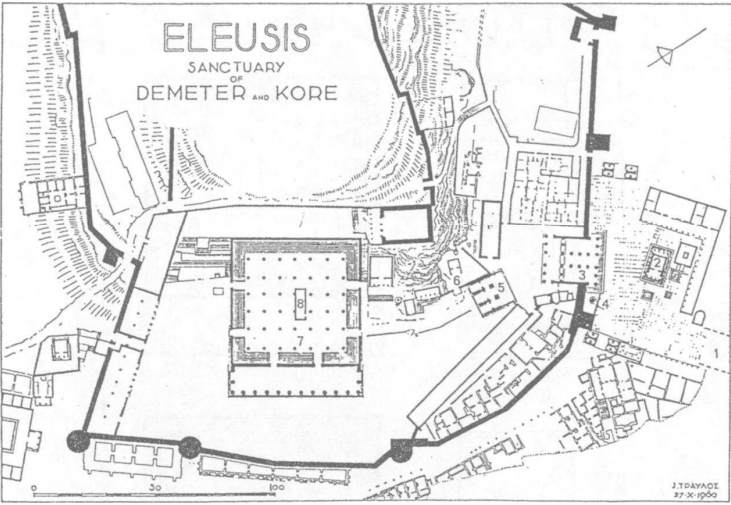
\includegraphics[width=0.6\linewidth]{Imagenes/PlanoSantuarioEleusis}
	\caption{\textit{\textit{Plano del recinto sagrado de Eleusis\footcite[231]{a.evansSanctuariesSacrificesEleusinian2002}}}}
	\label{fig:santuario de eleusis}
\end{figure}

\begin{figure}[h!]
	\centering
	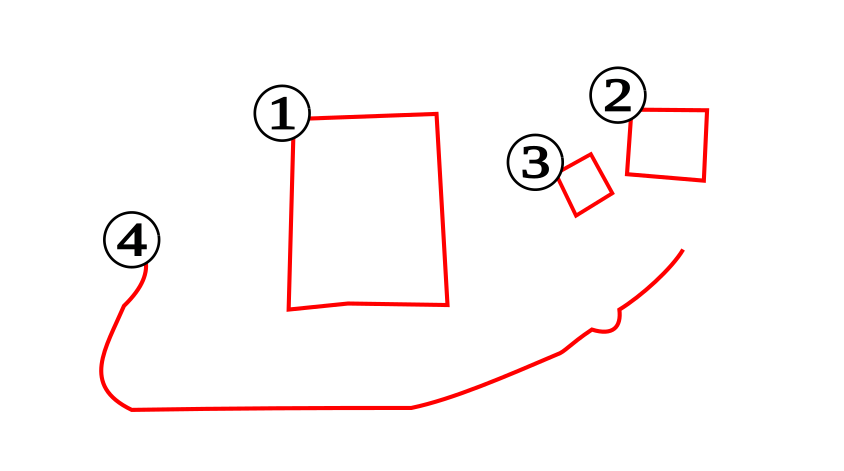
\includegraphics[width=0.6\linewidth]{Imagenes/VistaAereaEleusis}
	\caption{\textit{Vista Aérea. 1: Telesterion; 2: Propileo mayor; 3: Propileo menor; 4. Muro del temenos; 5. Anaktoron. Google Earth}}
	\label{fig:vista aérea del santuario de eleusis}
\end{figure}





\section{Símbolos e iconografía}

Los principales elementos simbólicos del culto de Eleusis eran el kykeon (la bebida) y la \textit{kíste} o \textit{cista mystica}. También eran muy característicos el mirto y el trigo. 
La kíste era una cesta cubierta con una tapa y en ocasiones se representaba con una serpiente rodeándola, signo de lo que es 'indecible'.

Estos elementos, aparecen habitualmente en las representaciones artísticas relacionadas con los misterios. El kykeon, al tratarse de una bebida, venía representado con una copa metálica de la que se bebería la bebida sagrada.

\begin{figure}[h!]
	\centering
	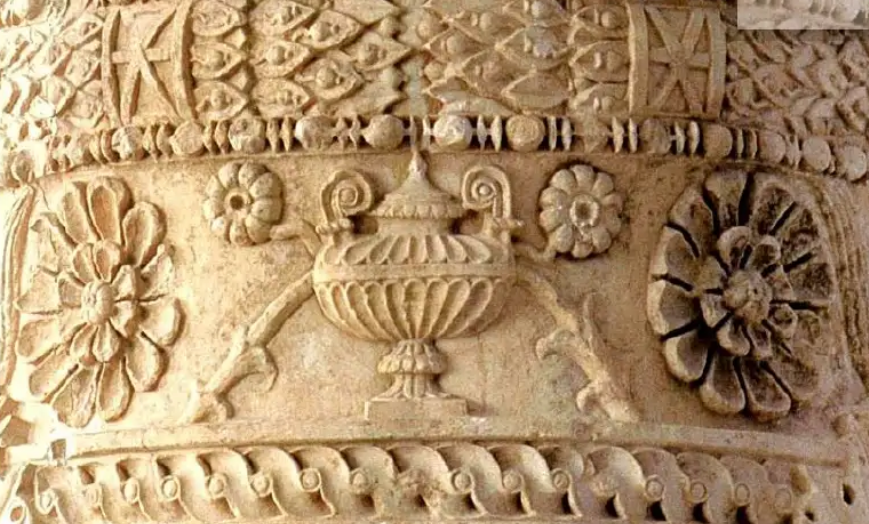
\includegraphics[width=0.45\linewidth]{Imagenes/CopaKykeon}
	\caption{\textit{Representación de la copa metálica destinada al kykeon, perteneciente a la cista mystica que portaban en la cabeza las cariátides del propileos del recinto sagrado de Eleusis\footcite[35]{calvosorianoMisteriosEleusisImagenes2022}.}}
	\label{fig:copa kykeon cariatides}
\end{figure}

\begin{figure}[h!]
	\centering
	\includegraphics[width=0.45\linewidth]{Imagenes/CariátidesEleusis}
	\caption{\textit{Cariátide del propileo menor de Eleusis con la cista mystica en la cabeza (s. I a. C.).  Fotografía de George E. Koronaios\footcite[]{koronaiosCaryatidLesserPropylaia2018}.}}
	\label{fig:cariatides propileo menor}
\end{figure}

En este punto haremos una descripción de una serie de obras en las que podremos apreciar la iconografía de los misterios eleusinos. Para ello, describiremos a grandes rasgos la iconografía de ambas diosas. 

A Deméter se le solía representar como una mujer madura. Normalmente portando una corona y con un manojo de trigo, aunque también podía llevar una cornucopia y/o una antorcha. Sus animales atributos eran la serpiente y el cerdo. De hecho, ambos tienen presencia en los misterios eleusinos. En cuanto a Perséfone, se presentaba como una joven diosa sosteniendo también manojos de grano y una antorcha encendida. 

La Tablilla de Ninnio (Figura 2.5), encontrada en Eleusis, es de gran relevancia para el conocimiento de los misterios eleusinos, ya que nos muestra como debía ser la procesión hacia Eleusis. El desfile que aparece en ella esta organizado compositivamente en dos hileras: superior e inferior.

\begin{figure}[h!]
	\centering
	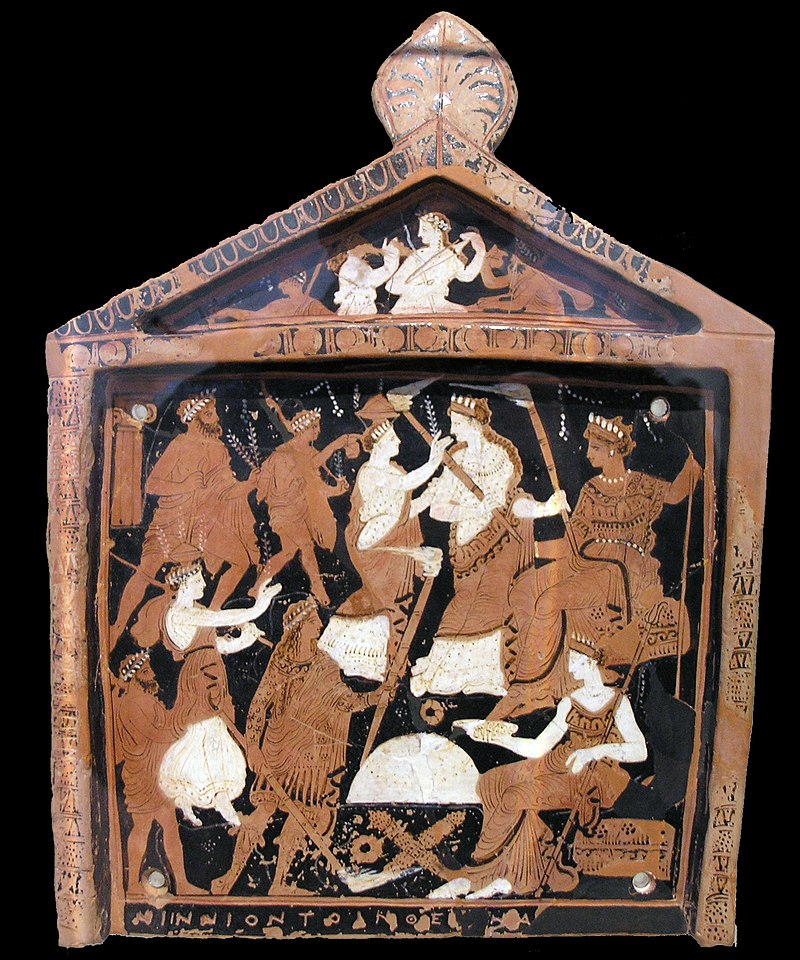
\includegraphics[width=0.45\linewidth]{Imagenes/TablillaDeNinnio}
	\caption{\textit{Tablilla de Ninnio (s. IV a. C.), Museo Arqueológico Nacional de Atenas.}}
	\label{fig:tablilla de Ninnio}
\end{figure}

En ella, aparecen Yaco y Hécate, cumpliendo el papel de daducos encabezando la procesión con sus antorchas en mano. Deméter aparece sentada en la roca llamada \textit{agelastos petra}; a su lado, se observa un trono vacío que seguramente estaba destinado a que lo ocupase Perséfone -también podría ser la cista mystica-, la cual aparece sentada al fondo de la imagen, ocupando su puesto como reina del Hades\footcite[105-106]{kerenyiEleusisImagenArquetipica2004}. 

Vemos que aparece un muchacho; se trata del 'muchacho del hogar', quien escogido en sorteo por los ciudadanos de Atenas para que fuera iniciado a expensas del estado en estos misterios , era el encargado de diferentes labores en el desarrollo del culto. Este realizaba las acciones sagradas en nombre de la comunidad\footcite[105]{kerenyiEleusisImagenArquetipica2004}. Aparece en la fila superior ocupando el segundo puesto desde la izquierda. 

Ninnio es el nombre de la mujer que dedicó esta tablilla a las dos diosas, de hecho esta cuenta con una inscripción en la que dice: "Ninnio se lo ha ofrecido a las Dos Diosas"; la mujer seguramente sea la que aparece representada en el frontón de la tablilla votiva. Sobre el suelo aparecen dos ramas de mirto cruzadas bajo la \textit{agelastos petra}, símbolo característico de los misterios. Los \textit{mystai} visten ropas oscuras, costumbre que se dejó de realizar en el siglo II, porque se comenzaron a usar vestimentas blancas, seguramente por influencia egipcia\footcite[107]{kerenyiEleusisImagenArquetipica2004}. 

De gran relevancia es también el relieve de mármol(Figura 2.2) en el que aparecen las dos diosas junto a Triptólemo. El relieve original data del siglo V a. C. y seguramente perteneciese al templo de Triptólemo. En él, podemos observar a las dos diosas, Deméter a la izquierda y Perséfone a la derecha. Perséfone porta una antorcha y Deméter le otorga una espiga de trigo a Triptólemo\footcite[139]{kerenyiEleusisImagenArquetipica2004}. 

\begin{figure}[h!]
	\centering
	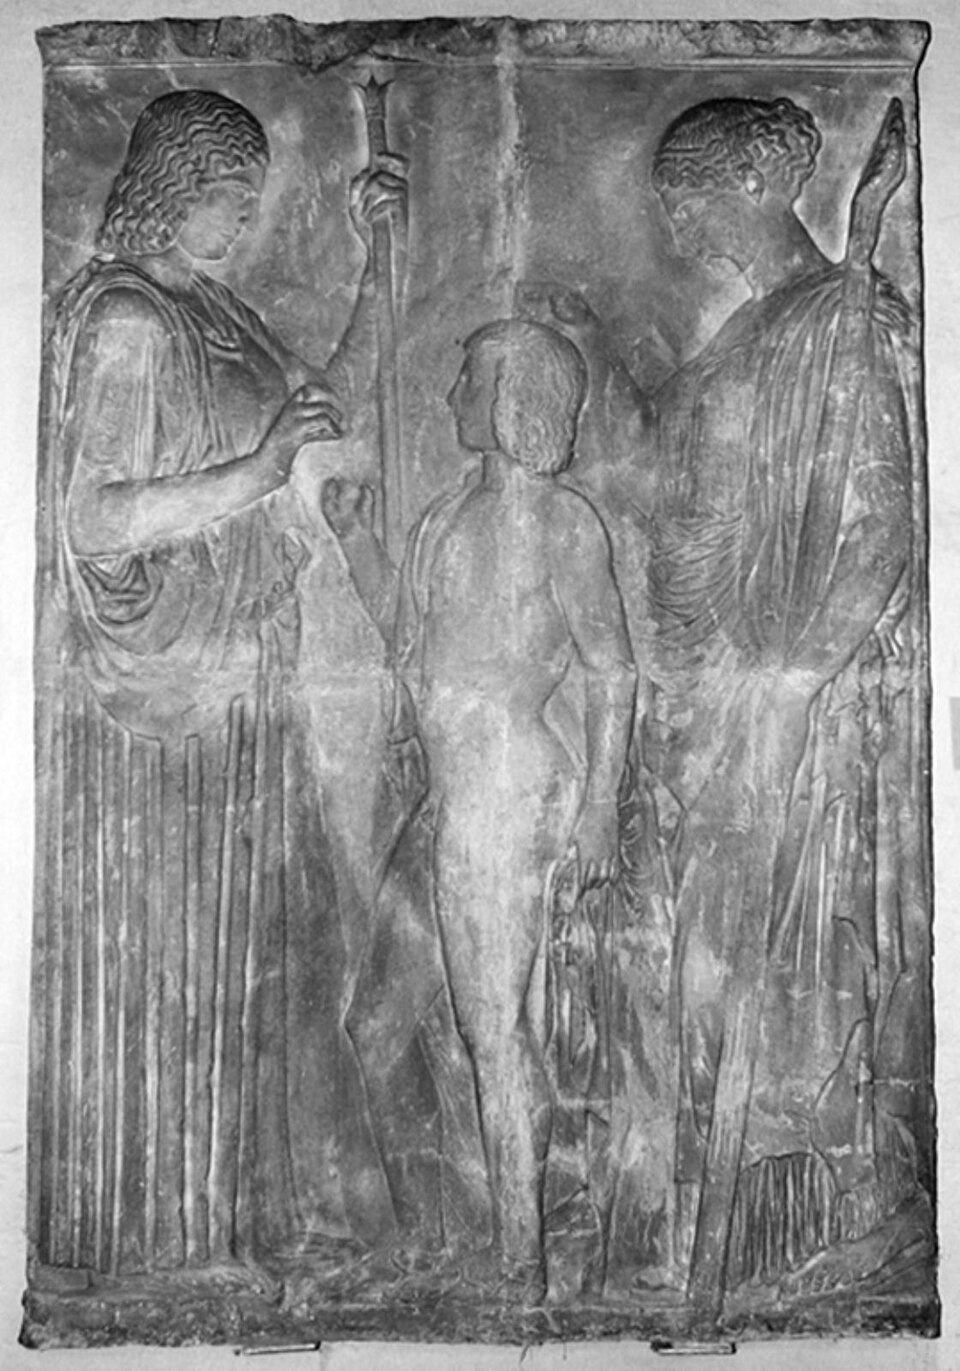
\includegraphics[width=0.45\linewidth]{Imagenes/RelieveDosDiosasTriptolemo}
	\caption{\textit{Relieve en mármol de Deméter, Perséfone y Triptólemo (s. V a. C.), Galería Nacional de Dinamarca (copia).}}
	\label{fig:relieve de las dos diosas y triptólemo}
\end{figure}


Por último, una urna cineraria romana descubierta en los mausoleos ubicados en la Puerta Mayor de Roma, cuyos relieves represetan los misterios. En ella, aparece Deméter con una corona de trigo sentada en la \textit{kisté} o cista mystica. Una serpiente se enrolla alrededor de esta. Kore aparece detrás de su madre sujetando una antorcha. También aparece un iniciado cubierto por un velo y con un cuerno de carnero bajo sus pies. A su espalda, se enuentra una sacerdotisa sujetando un \textit{liknon} (herramienta para separar la espiga del trigo) sobre la cabeza del \textit{mystai}. Por último, el relieve nos muestra a Hércules vestido con piel de león sujetando un cerdo para el sacrificio; mientras, un sacerdote (personaje a la izquierda con gran barba) sujeta una bandeja con ofrendas mientras está realizando una libación\footcite[94-94]{burkertAncientMysteryCults1987}. 
\begin{figure}[h!]
	\centering
	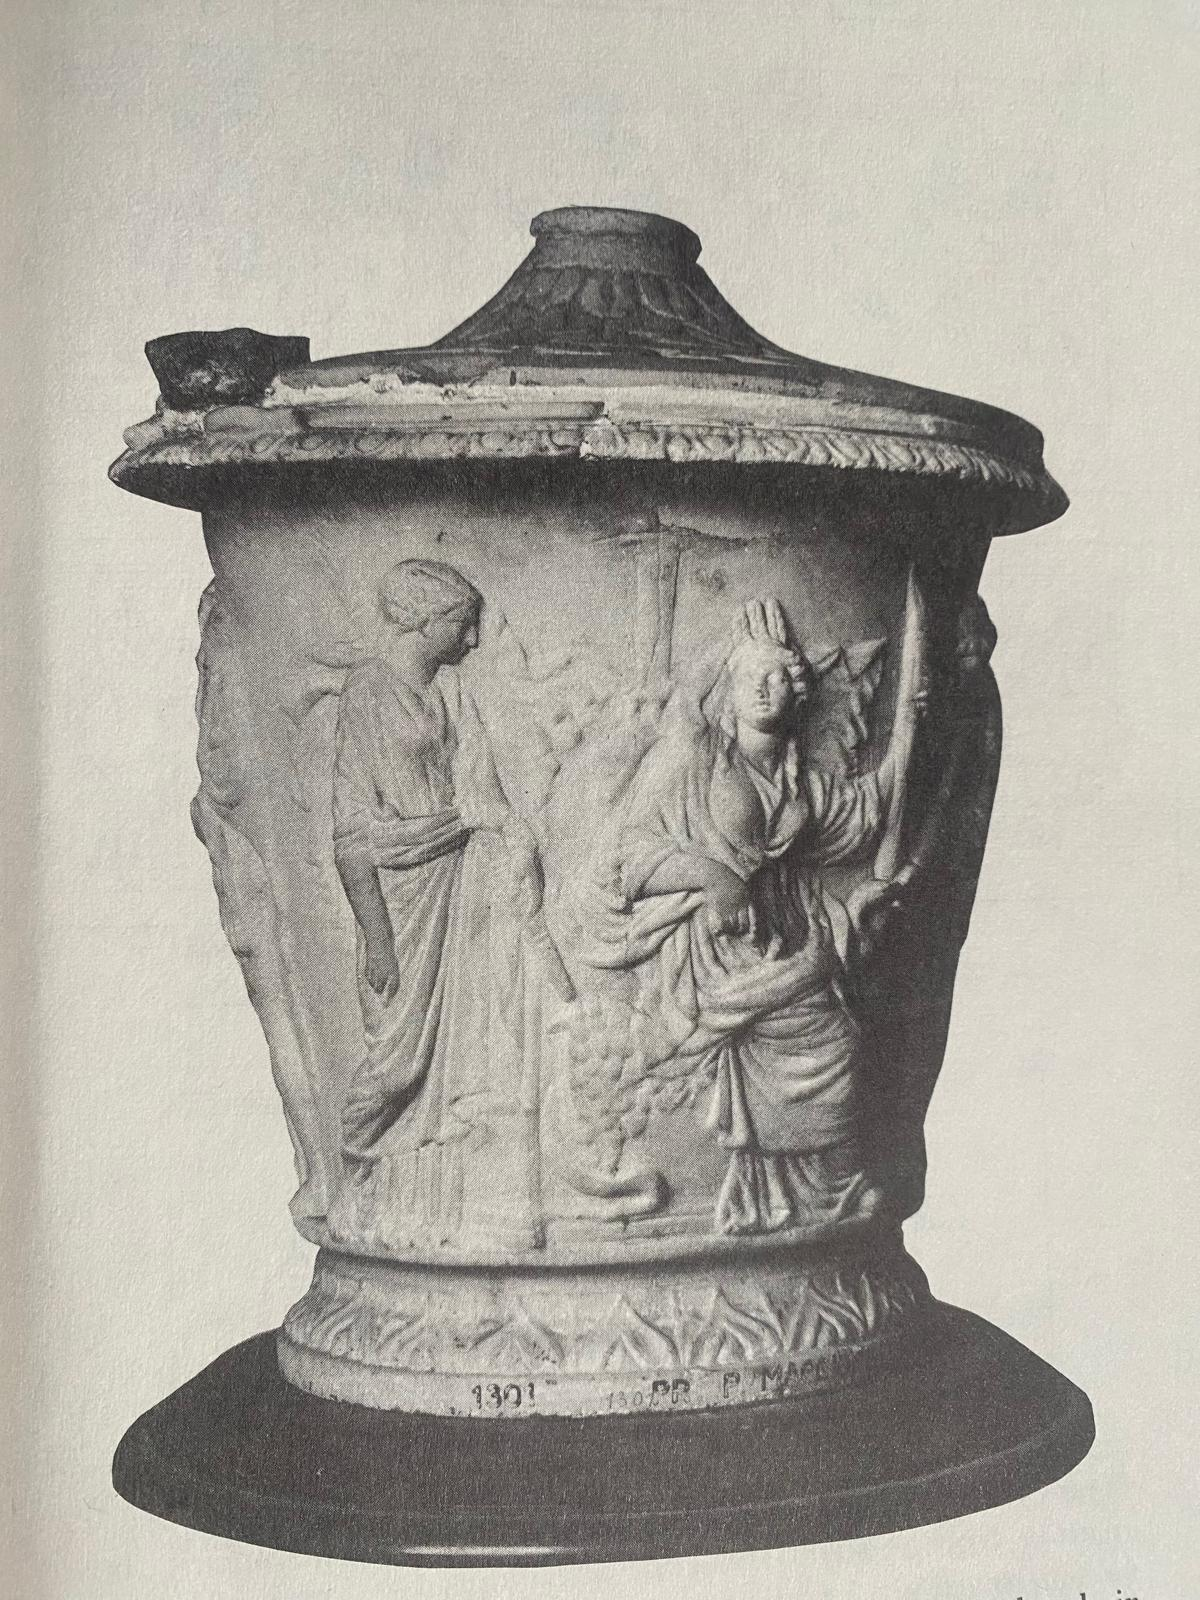
\includegraphics[width=0.45\linewidth]{Imagenes/Urna1}
	\caption{Urna Caetani Lovatelli (s I a. C.), Museo Nacional Romano \footcite[53-66]{burkertAncientMysteryCults1987}.}
	\label{fig:urna-1}
\end{figure}

\begin{figure}[h!]
	\centering
	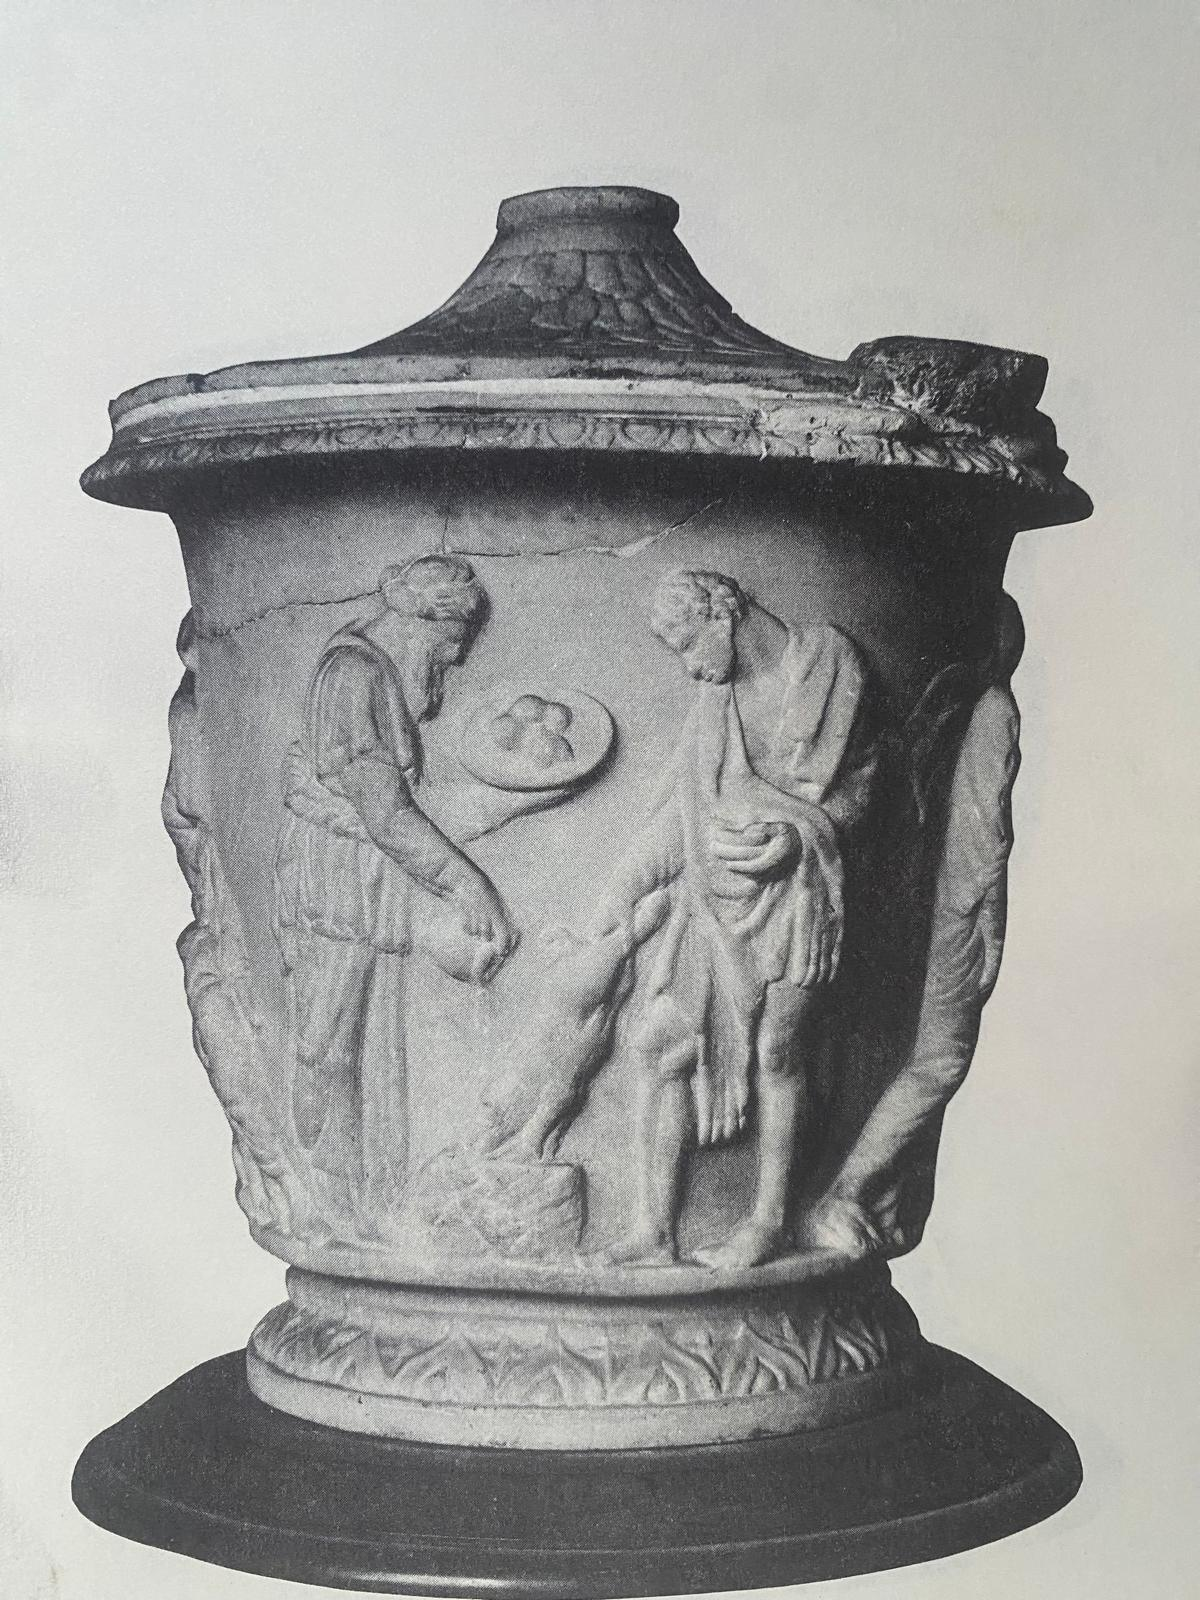
\includegraphics[width=0.45\linewidth]{Imagenes/Urna3}
	\caption{Urna Caetani Lovatelli (s. I a. C.), Museo Nacional Romano \footcite[53-66]{burkertAncientMysteryCults1987}.}
	\label{fig:urna-3}
\end{figure}

\begin{figure}[h!]
	\centering
	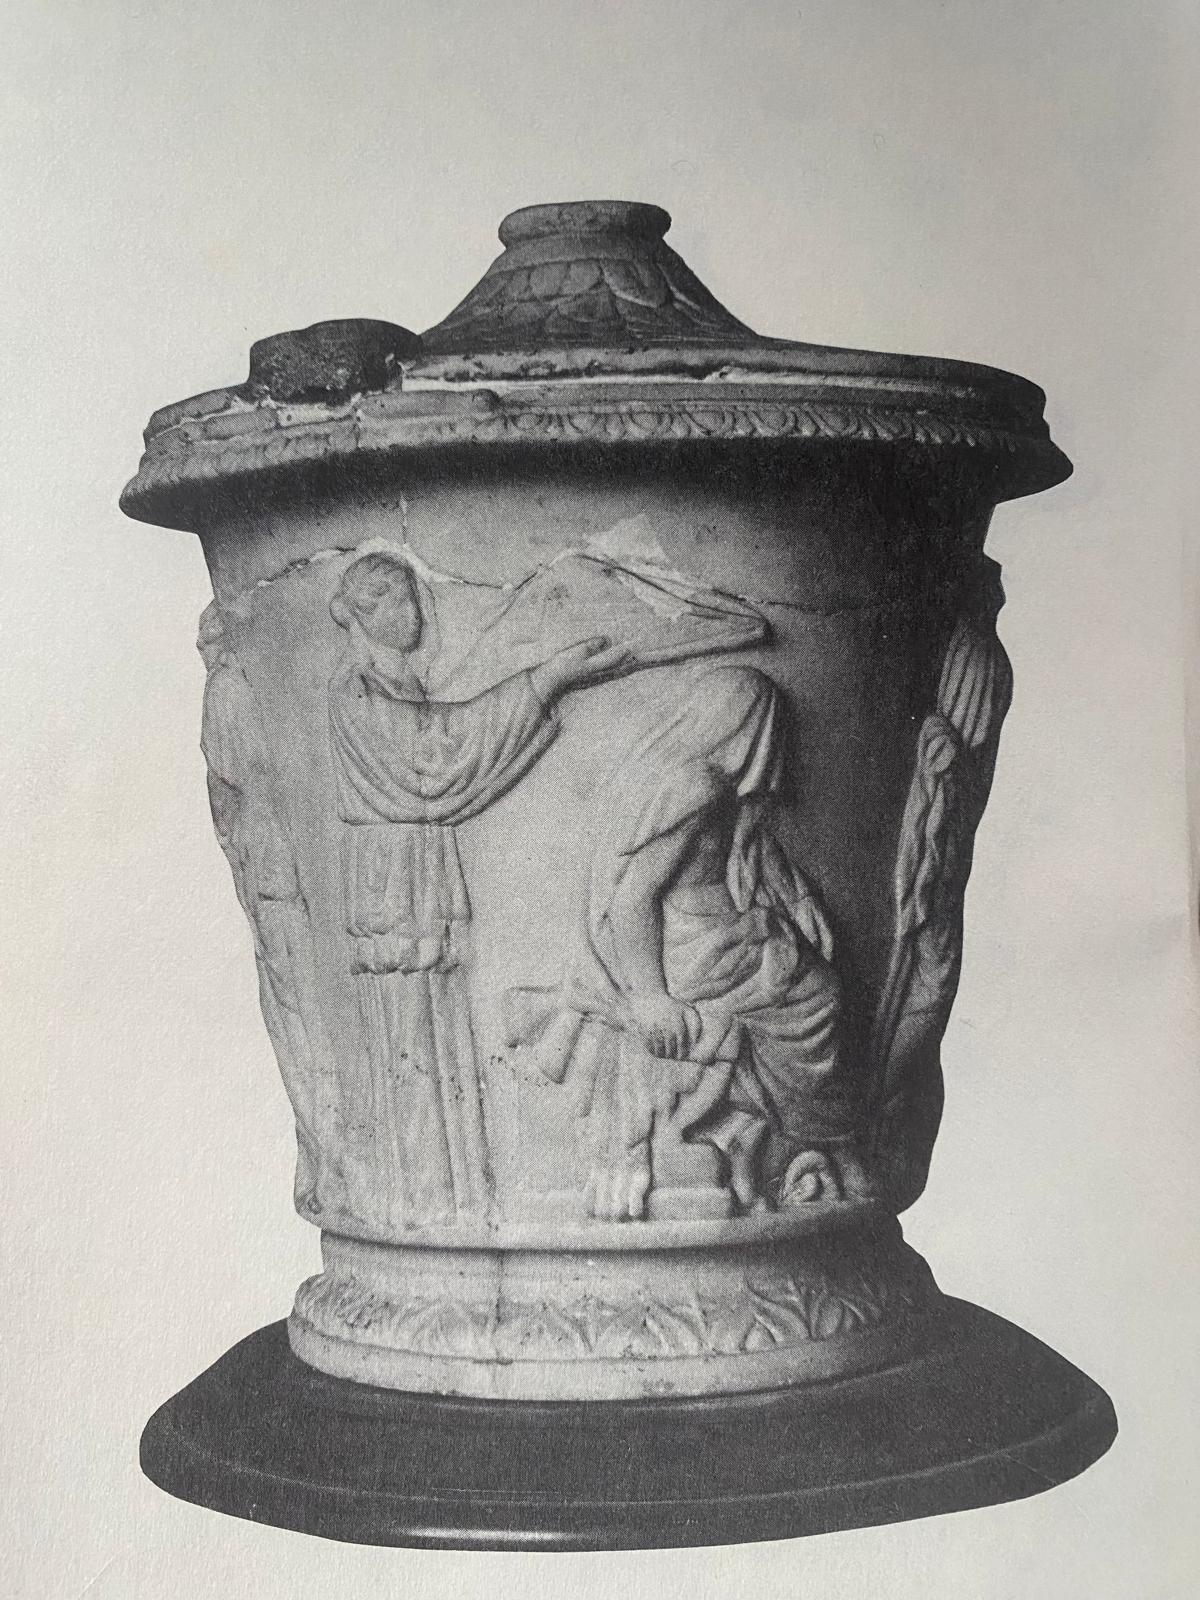
\includegraphics[width=0.45\linewidth]{Imagenes/Urna2}
	\caption{Urna Caetani Lovatelli (s. I a. C.), Museo Nacional Romano \footcite[53-66]{burkertAncientMysteryCults1987}.}
	\label{fig:urna-2}
\end{figure}


\section{Función y significado de los misterios eleusinos}

Burkert señala la doble existencia de Deméter entre el mundo superior y subterráneo, presentando dos dimensiones de \textit{"muerte en vida y de vida en la muerte"} \footcite[310]{burkertReligionGriegaArcaica2007}, siendo entonces Deméter una divinidad ctónica. Además, los atenienses llamaban Demétreioi a los muertos y sembraban grano en sus tumbas. Este hecho señala una doble funcionalidad relacionada con el trigo como sustento vital dotado por Deméter y la pérdida del miedo a la muerte en relación con Perséfone. En definitiva, dando un sentido esperanzador al fin de la existencia humana. Esta función de Perséfone está relacionada con la superación del individuo de su miedo al 'más allá', es decir, a la muerte. Marvin Meyer también indica esa misma dualidad funcional presentando a las dos diosas; Deméter como personificación del grano y Perséfone como la reina del Hades \footcite[12]{w.meyerAncientMysteriesSource1986}. Entonces podríamos establecer una doble funcionalidad, una relacionada con las cosechas y el trigo como fuente de sustento, y otra, en relación al más allá y la superación del miedo a la muerte.

Kerenyi, en su estudio, mantiene que los misterios de Eleusis mantenían unida a toda la comunidad. La iniciación en Eleusis otorgaba confianza ante la muerte, función que actuaba desde la dimensión individual hasta la comunitaria, y por eso establece que los misterios debían estar relacionados con la existencia humana \footcite[31]{kerenyiEleusisImagenArquetipica2004}. Como ejemplo, muestra el texto de Heródoto (que hemos mostrado en el apartado de Desarrollo del culto), en el que en medio de una guerra con Persia, los ciudadanos recurren a los misterios eleusinos en busca de salvación de grecia como comunidad.

Kerenyi recurre también a los términos de 'bienaventuranza' y 'beatitud' (términos cristianos), para describir lo que los \textit{mystai} podían experienciar al realizar las ceremonias iniciáticas. La 'bienaventuranza' interior se trataba de la beatitud que conseguía el iniciado, entendiendo este concepto como el estado de dicha una vez traspasada la frontera hacia el 'más allá'. Pero siguiendo con la dualidad funcional, también existía una 'bienaventuranza' exterior, que es la riqueza del grano.

La iniciación se formula como un rito de tránsito que concedía el paso de una 'categoría' a otra con sentido más especial. Era el camino para conseguir la madurez en cada uno de los aspectos tratados en el rito. En el caso de los misterios, se le otorga al iniciado el \textit{"tránsito de la indiferencia a la gracia"} \footcite[156]{reyesReligionGriega2018}. El término 'gracia', mencionado en estas palabras de Alfonso Reyes, se refiere a lo mismo que nos dice Kerenyi sobre la 'beatitud' de los iniciados. 
Ya hemos dicho que hombres y mujeres podían participar en los misterios, ya que estos muestran la imagen arquetípica de la separación entre madre e hija. Esta separación marca la existencia de hombres y mujeres, aunque seguramente de diferente manera. En la \textit{epopteia} ambos llegaban a la contemplación de las imágenes divinas. El factor universalizante del culto, según Kerenyi, era el origen femenino de la vida \footcite[158]{kerenyiEleusisImagenArquetipica2004}, que afectaba tanto a hombres como mujeres. De igual manera tenía importancia la espiga del grano como símbolo del don que Deméter concede a los humanos 

Nos interesa comentar también la visión de Cosmopoulos. En ella, los misterios son una forma de lidiar con los dioses de la polis de una forma individual, ya que cuando el iniciado realizaba su ritual, tenía el poder de compartir la verdad eterna. Los ciudadanos veían los misterios como una manera de lidiar con su propia mortalidad. \footcite[]{cosmopoulosGreekMysteriesArchaeology2005}. 

Recapitulando; los misterios eleusinos surgen como una manera de luchar contra la propia mortalidad desde una dimensión individual. Nacen de una necesidad espiritual de los ciudadanos que la religión oficial ya no podía satisfacer. En este caso, los misterios eleusinos dotan de las riquezas que las dos diosas representan: el sustento natural y la bienaventuranza en el más allá. 